\documentclass[a4paper]{article}
\linespread{1.5}
\usepackage{graphicx} % Required for inserting images
\usepackage{xeCJK}
\usepackage[utf8]{inputenc} 
\usepackage{amsmath,amssymb,amsfonts,mathrsfs,latexsym,amsthm}
\usepackage{ulem}
\usepackage{graphicx}
\usepackage{titlepic}
\usepackage{enumerate}
\usepackage{enumitem}
\usepackage{float}
\usepackage{gensymb} %温度符号
\usepackage[margin=1.0in]{geometry}
\usepackage{titlesec}
\usepackage{hyperref}


%bibLatex(引用)
\usepackage[
backend=bibtex,
]{biblatex}
%Table(表格)
\usepackage[table,xcdraw]{xcolor}
\usepackage{longtable}

%图形
\usepackage{pstricks}
%\usepackage{ntheorem}
\usepackage{pgfpages}
%\pgfpagesuselayout{4 on 1}[a4paper,border shrink=5mm]
%\usepackage{floatflt}
%pakke til at lave sætningsenvorinmets (kan ikke loades sammen med amsthm)
\usepackage{tikz}

%电路图
\usepackage{fontawesome}
\usepackage{pgf}
\usepackage{mathrsfs}
\usetikzlibrary{arrows}
\usepackage{multicol}
\usepackage{multirow}

%化学
\usepackage[version=4]{mhchem}

%定理,证明环境
\theoremstyle{definition}
\newtheorem{definition}{Definition}[section]
\newtheorem{sætning}[definition]{Sætning}
\newtheorem{hypothesis}[definition]{Hypotese}
\newtheorem*{bemærkning}{Bemærkning}

%页码,页脚页眉
\usepackage{fancyhdr}
\usepackage{lastpage}
\fancyhf{}
\lhead{{CSN F9} \\ {飞行机组操作手册}}
\rfoot{第\hspace{1pt} \thepage \hspace{1pt} 页}

\newlength{\evenmarginwidth}
\setlength{\evenmarginwidth}{\evensidemargin+2em}
\fancyhfoffset{\evenmarginwidth}

%CC license
\usepackage[
type={CC},
modifier={by},
version={4.0},
]{doclicense}

%文字填充
\usepackage{zhlipsum}

%自定义命令
\newcommand{\checklistline}[3][1]{\hspace{{#1}em}{#2} \dotfill\ {#3}}
\newcommand{\checklistlinewithast}[3][1]{\hspace{{#1}em}{$^{\ast}${#2}} \dotfill\ {#3}}
\newcommand{\checklisttext}[2][1]{\vspace{0.75em}\hspace{{#1}em}\parbox{\textwidth-{#1}em}{#2}\vspace{0.75em}}
\newcommand{\textbox}[1]{\hspace{-2em}\framebox[\textwidth+4em]{\textbf {#1}}}
\newcommand{\DUtitle}[1]{{\hspace{-1em}\textbf{\uline{#1}}}}

\newcommand{\cll}[3][1]{\hspace{{#1}em}{#2} \dotfill\ {#3}}
\newcommand{\astcll}[3][1]{\hspace{{#1}em}{$^{\ast}${#2}} \dotfill\ {#3}}
\newcommand{\clt}[2][1]{\vspace{0.75em}\hspace{{#1}em}\parbox{\textwidth-{#1}em}{#2}\vspace{0.75em}}



%关闭段落起始缩进
\setlength{\parindent}{0em}
\setlength{\hoffset}{1em}



\begin{document}		
%封面
\begin{titlepage}
	\begin{center}
		\vspace{1cm}
		{\color{F9blue}{\Huge \textbf{{ CSN F9「碳箭」}}}}\\
		\vspace{1.5cm}
		{\Large \textbf{{飞行机组操作手册}}}\\
		\vspace{2.5cm}
		\begin{center}
			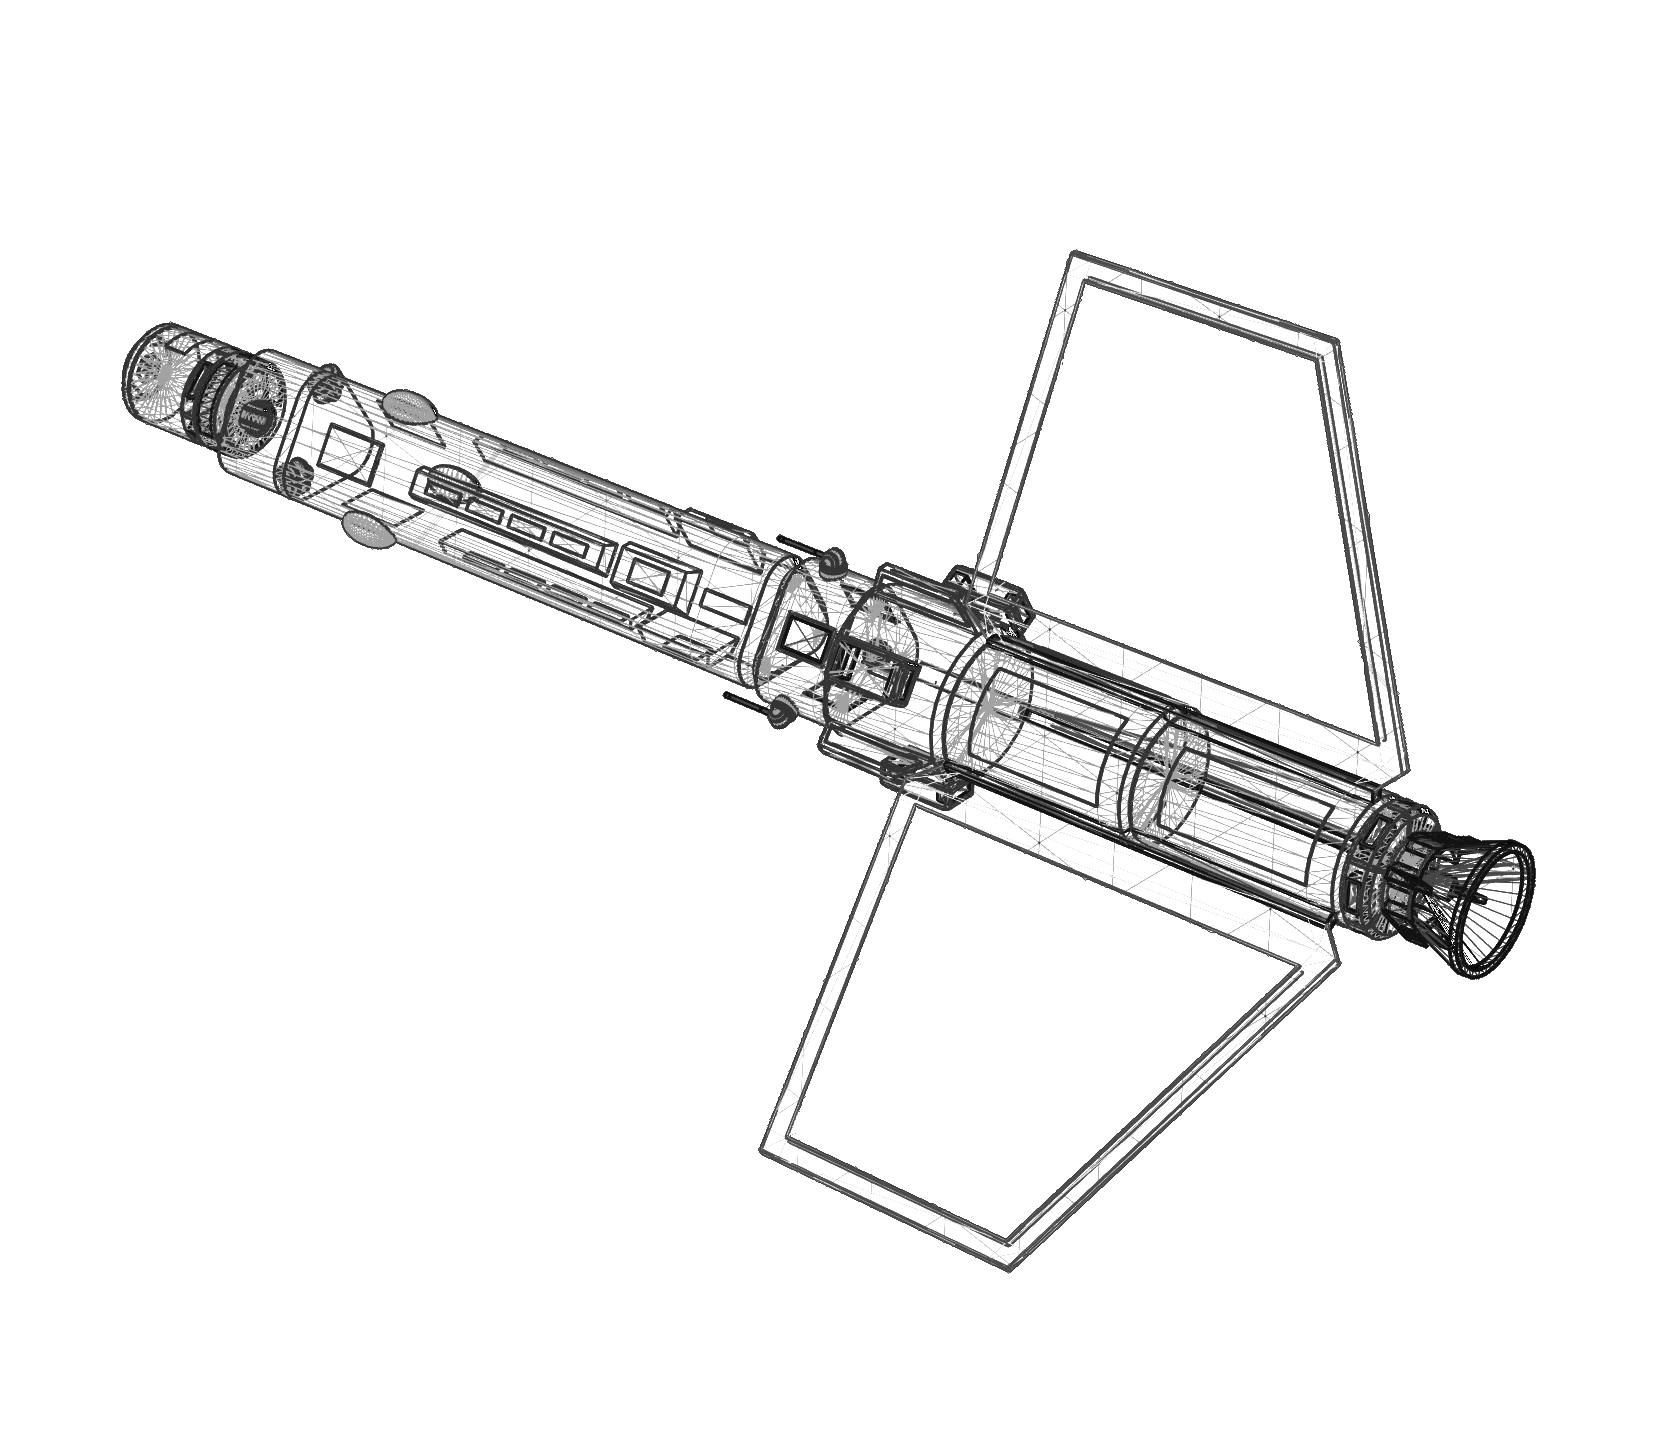
\includegraphics[width=0.7\linewidth]{Picture/F9_titlepic}
		\end{center}
		\vfill
		\vspace{1.8cm}
		\doclicenseThis
	\end{center}
\end{titlepage}
\newpage

%页脚页眉初始化
\pagenumbering{arabic}
\pagestyle{fancy}
\setcounter{page}{1}

%目录
\renewcommand*\contentsname{目录}
\tableofcontents
\newpage



%正文
\addcontentsline{toc}{section}{GEN 综合信息}
\section*{{\hspace{-1em}综合信息}}
\addcontentsline{toc}{subsection}{术语表}
\hspace{-2em}\framebox[\textwidth+4em]{\textbf {术语表}}
 
\vspace{10pt}
{\hspace{-1em}\textbf{\uline{导航}}}
{\small{
\begin{longtable}{|p{4.5cm}|p{\textwidth-6.5cm}|}
	\hline
	Nav                             & 导航      \\ \hline
	Navigation                      & 导航      \\ \hline
	Maneuvers                       & 机动      \\ \hline
	Mvr                             & 机动      \\ \hline
	Jumps                           & 跳跃      \\ \hline
	flight plan                     & 飞行计划    \\ \hline
	Flight Planning                 & 飞行规划    \\ \hline
	Prograde                        & 顺向      \\ \hline
	apoapsis                        & 远拱点     \\ \hline
	periapsis                       & 近拱点     \\ \hline
	Plane                           & 平面      \\ \hline
	Burn                            & 点火      \\ \hline
	DeltaV                          & 速增量     \\ \hline
	Translation                     & 平移      \\ \hline
	guidance                        & 制导      \\ \hline
	Jump-Space                      & 跳跃空间    \\ \hline
	Jump-Space polarization         & 跳跃空间极化  \\ \hline
	jump-point                      & 跳跃点     \\ \hline
	Modulation                      & 调制      \\ \hline
	Course Correction               & 航线修正    \\ \hline
	trajectory propagator           & 轨迹预报模型  \\ \hline
	Routine                         & 例程      \\ \hline
	NavTask                         & 导航任务    \\ \hline
	Route                           & 航路      \\ \hline
	Route Finder                    & 航路查询器   \\ \hline
	refueling stop                  & 经停加注    \\ \hline
	Navigation Station              & 导航站     \\ \hline
	Automatic Flight Planner        & 自动飞行规划器 \\ \hline
	Flight Editor                   & 飞行编辑器   \\ \hline
	Flight Analyzer                 & 飞行分析器   \\ \hline
	Jump Explorer                   & 跳跃浏览器   \\ \hline
	Sweep                           & 扫掠      \\ \hline
	leg                             & 航节      \\ \hline
	segment                         & 航段      \\ \hline
	ringed planets                  & 有环行星    \\ \hline
	ring station                    & 星环空间站   \\ \hline
	true anomaly                    & 真近点角    \\ \hline
	encounter                       & 交会      \\ \hline
	celestial body                  & 天体      \\ \hline
	Orbital Elements                & 轨道根数    \\ \hline
	Epoch                           & 历元      \\ \hline
	semi major axis                 & 半长轴     \\ \hline
	eccentricity                    & 离心率     \\ \hline
	inclination                     & 倾角      \\ \hline
	longitude of the ascending node & 升交点经度   \\ \hline
	lan                             & 升交点经度   \\ \hline
	argument of the periapsis       & 近心点辐角   \\ \hline
	tra                             & 真近点角    \\ \hline
	rms                             & 均方根     \\ \hline
	rms                             & 均方根误差   \\ \hline
	Dilution of Precision           & 精度衰减因子  \\ \hline
	Dead Reckoning                  & 航位推算法   \\ \hline
	planned trajectory              & 预定轨迹    \\ \hline
	radio emission                  & 射电辐射    \\ \hline
	ETE                             & 预计航路时间  \\ \hline
	SOI                             & 影响球     \\ \hline
	Coordinated Galactic Time       & 协调银河时   \\ \hline
	B-Plane                         & B 平面    \\ \hline
	Intercept                       & 拦截      \\ \hline
	Propagation                     & 预报      \\ \hline
	jump approach                   & 跳跃点进近   \\ \hline
	intermediate orbit              & 中间轨道    \\ \hline
	agp                             & 近点辐角    \\ \hline
	sma                             & 半长轴     \\ \hline
	ecc                             & 离心率     \\ \hline
	peD                             & 近拱点距    \\ \hline
	apD                             & 远拱点距    \\ \hline
	inc                             & 倾角      \\ \hline
	Orbital period                  & 轨道周期    \\ \hline
	jump-point locator              & 跳跃点定位标  \\ \hline
	ETA                             & 预达时间    \\ \hline
	RDV                             & 会合      \\ \hline
	Rendez-vous                     & 会合      \\ \hline
	Clearance                       & 净空      \\ \hline
\end{longtable}}}
\newpage










\hspace{-2em}\framebox[\textwidth+4em]{\textbf {冷启动}}


{\hspace{-1em}\textbf{\uline{电气系统}}}

\checklistline{重要汇流条电压}{检查}

\checklistline{ESSPU 电池充电}{检查}

\checklistline{ESCU 电池电量}{检查}

\checklistline{SRPS1电门}{接通}

\checklistlinewithast{港口电源电门}{ON}

\vspace{0.75em}\hspace{1em}\parbox{\textwidth-1em}{将主汇流条接入空间站电网。
	注意:空间站侧的供电(400 V 和 21 kV)可通过
	『轨道服务』界面控制。默认两路
	均开启。}\vspace{0.75em}
	
	外部绕机检查确保飞机整体状态、可视部件和设备对于飞行是安全的。
	每次首次飞行前,通常维护人员做全面检查,如果维护人员不在,可由飞行机组完
	成。
	

\textbox{热启动}
\checklisttext[3]{将主汇流条接入空间站电网。注意:空间站侧的供电(400 V 和 21 kV)可通过}

\end{document}
